%%%%%%%%%%%%%%%%%%%%%%%%%%%%%%%%%%%%%%%%%%%%%%%%%%%%%%%%%%%%%%%%%%%%%%%%%%%

\documentclass{standalone}

\usepackage{amsmath}
\usepackage{mathptmx}
\usepackage{pgfplots}
\usetikzlibrary{external}
\tikzexternalize{Australia-gdp-per-capita-delta}
\pgfplotsset{compat=1.16}

%% IEEE uses Times Roman font, so we'll default to Times.
%% These three commands make up the entire times.sty package.
\renewcommand{\rmdefault}{ptm}
\renewcommand{\ttdefault}{pcr}
\normalfont\selectfont

\begin{document}

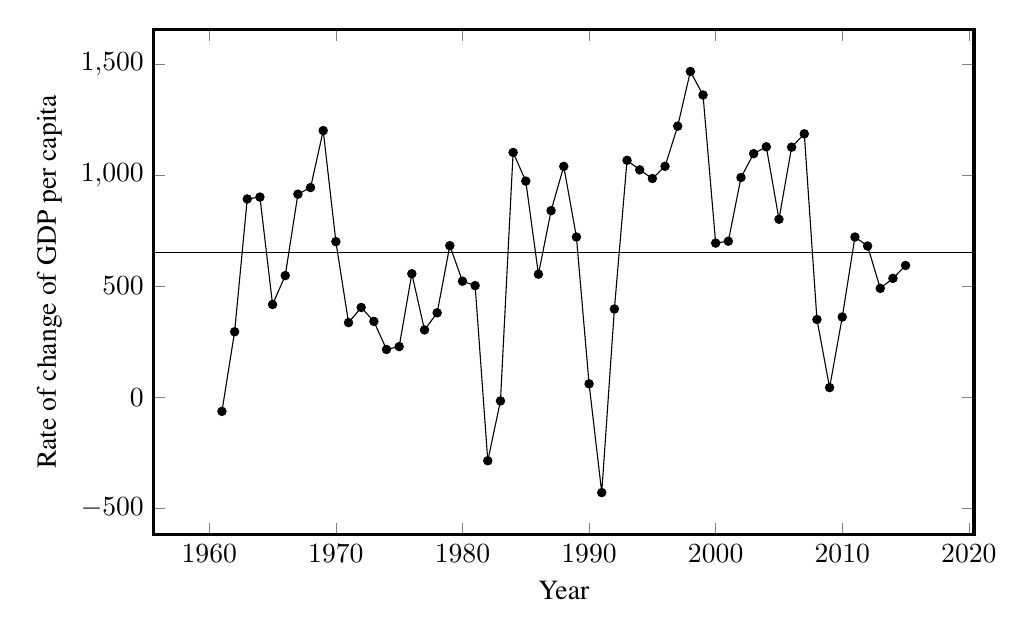
\begin{tikzpicture}
\tikzset{%%
  every mark/.append style={scale=1.0},%%
  scale=1.0%%
}
\pgfplotsset{%%
  every axis/.append style={font=\normalsize}%%
}
%%
\begin{axis}[%%
  axis line style=very thick,%%
  dotStyle/.style={mark size=1.5,black,mark color=black,mark=*},%%
  enlargelimits=true,%%
  height=8cm,%%
  width=12cm,%%
  %% x axis
  xlabel={\normalsize Year},%%
  xtick={1960,1970,1980,1990,2000,2010,2020},%%
  xticklabels={$1960$,$1970$,$1980$,$1990$,$2000$,$2010$,$2020$},%%
  %% y axis
  ylabel={\normalsize Rate of change of GDP per capita}%%
]
%%
%%
%% Horizontal line through the mean.
\draw[ultra thin] (axis cs:\pgfkeysvalueof{/pgfplots/xmin},650.707041295223) -- (axis cs:\pgfkeysvalueof{/pgfplots/xmax},650.707041295223);
%%
%%
\addplot[dotStyle] coordinates {
  (1961, -64.2309824535387)
  (1962, 294.037178663129)
  (1963, 891.547446857934)
  (1964, 900.279073357462)
  (1965, 416.903339083634)
  (1966, 546.872379667884)
  (1967, 913.193439477058)
  (1968, 943.044726876502)
  (1969, 1199.41424201567)
  (1970, 699.655777498707)
  (1971, 335.226046680569)
  (1972, 403.282748447344)
  (1973, 340.731933798623)
  (1974, 214.298465413387)
  (1975, 227.438665096031)
  (1976, 555.172519247288)
  (1977, 302.206800931011)
  (1978, 379.349372274024)
  (1979, 681.561812445909)
  (1980, 521.580157006727)
  (1981, 501.728963810998)
  (1982, -286.531170957865)
  (1983, -17.2752676969467)
  (1984, 1100.95878699026)
  (1985, 972.113170622944)
  (1986, 552.979607423404)
  (1987, 839.290580537459)
  (1988, 1038.31863543245)
  (1989, 720.421681144824)
  (1990, 59.6849262806863)
  (1991, -429.789497810947)
  (1992, 396.526672138589)
  (1993, 1065.64052677574)
  (1994, 1022.63403137076)
  (1995, 983.562802607597)
  (1996, 1038.71565124478)
  (1997, 1219.28575742936)
  (1998, 1465.55573470813)
  (1999, 1359.54766954542)
  (2000, 692.980944446441)
  (2001, 701.515397268562)
  (2002, 988.218289365963)
  (2003, 1095.63860046362)
  (2004, 1126.44475336633)
  (2005, 800.393543696886)
  (2006, 1124.86617227057)
  (2007, 1184.87691422731)
  (2008, 349.378109834175)
  (2009, 42.8201669734444)
  (2010, 360.465639986942)
  (2011, 720.474716700875)
  (2012, 679.92471597256)
  (2013, 489.382144777417)
  (2014, 534.181213204007)
  (2015, 592.391544699149)
};
\end{axis}
\end{tikzpicture}

\end{document}
